\chapter{Morpheus Spectral Counter: A Computational Tool for Label-Free Quantitative Mass Spectrometry using the Morpheus Search Engine}

\section{Summary}
Label-free quantitative MS based on the Normalized Spectral Abundance Factor (NSAF) has emerged as a straightforward and robust method to determine the relative abundance of individual proteins within complex mixtures.
Here, we present Morpheus Spectral Counter (MSpC) as the first computational tool that directly calculates NSAF values from output obtained from Morpheus, a fast, open-source, peptide-MS/MS matching engine compatible with high-resolution accurate-mass instruments.
NSAF has distinct advantages over other MS-based quantification methods, including a higher dynamic range as compared to isobaric tags, no requirement to align and re-extract MS1 peaks, and increased speed.
MSpC features an easy to use graphic user interface that additionally calculates both distributed and unique NSAF values to permit analyses of both protein families and isoforms/proteoforms.
MSpC determinations of protein concentration were linear over several orders of magnitude based on the analysis of several high-mass accuracy datasets either obtained from PRIDE or generated with total cell extracts spiked with purified \textit{Arabidopsis} 20S proteasomes.
The MSpC software was developed in C\# and is open sourced under a permissive license with the code made available at \url{http://dcgemperline.github.io/Morpheus_SpC/}. 

\section{Main Text}
Quantification of individual polypeptides within complex mixtures by MS is an extremely useful tool to understand proteomic changes in organisms during growth and development, and after environmental perturbation \citep{wong10}.
While a number of MS/MS strategies have been developed to measure protein abundance, including Stable Isotope Labeling by Amino Acids in Cell Culture (SILAC), labeling with isobaric tags, and Absolute Quantification of proteins (AQUA) \citep{gerber03, ong02, ross04, thompson03}, label-free quantification (LFQ) have become increasingly popular given their simplicity and low cost \citep{wong10, zhang06}.
One LFQ strategy infers abundance from the number of observed peptide spectra matches (PSMs).
For these PSM-based approaches, changes in protein abundance can be generated artifactually when total PSMs differ among samples and because longer proteins tend to produce more raw counts.
For these reasons normalizing for both protein length and total PSMs is paramount.
While this adjustment can be made in a number of ways; one of the most straight forward methods is to use Normalized Spectral Abundance Factor (NSAF), a length- and count-normalized measure for each protein \citep{zybailov06}.
Further improvements to the NSAF algorithm have been made by accounting for shared peptides in distributed NSAF (dNSAF), which distributes common PSMs among a family of isoforms/proteoforms based on the number of distinct PSMs observed for each isoform/proteoform, and unique NSAF (uNSAF), which ignores shared PSMs and only assigns distinct PSMs to each specific isoform/proteoform \citep{zhang10}.

The Morpheus MS search engine was recently designed for high-resolution, accurate-mass data obtained from Orbitrap-based instruments to provide faster matching of spectra to peptides \citep{wenger13}.
Unfortunately, no downstream automated tools are available to facilitate LFQ analysis, which can be quite challenging, if not impossible, to complete manually when accounting for shared peptides.
To overcome this bottleneck, we developed Morpheus Spectral Counter (MSpC) as the first LFQ computational tool that integrates directly with Morpheus to calculate NSAF, dNSAF, uNSAF, and corrected PSM \citep{fermin11} values in complex protein samples.
\begin{sidewaysfigure}[p]
	\centering
	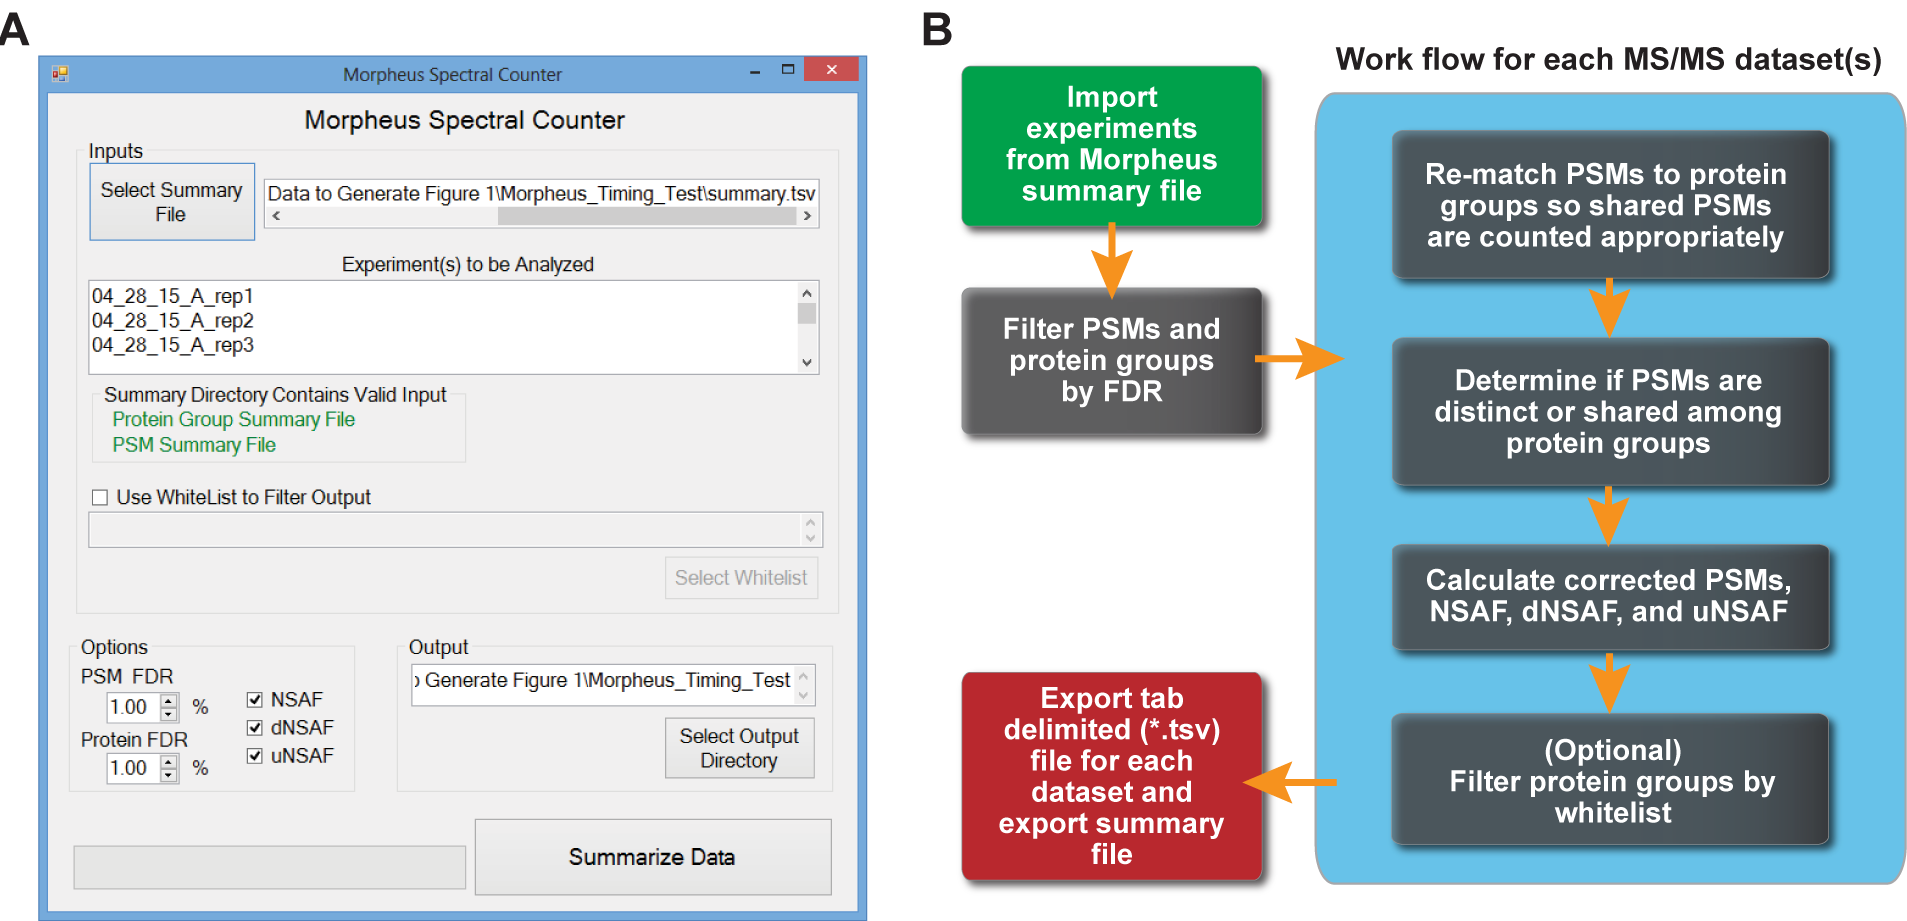
\includegraphics[width=\columnwidth]{MSpC/figure1_supplemental.png}
	\mycaption{MSpC Graphic User Interface (GUI) and software flow chart}{
\textbf(A) Screenshot of the GUI.
The input requires the user to select a Morpheus search summary file containing experiments to be analyzed.  The user can optionally select a whitelist to filter output, and select an output directory.
Additional options can set peptide and protein FDR cutoffs, and method of quantification for output, including Normalized Spectral Abundance Factor (NSAF), distributed NSAF (dNSAF), and unique	NSAF (uNSAF).
A progress bar highlights completion of the analysis.
\textbf(B) Data analysis flow chart.
Experiments and groups of experiments to be analyzed are imported through the Morpheus summary file.
PSMs and protein groups are filtered at the specified FDR cutoff with a default of 1\%.}
	\label{fig:GUIflow}
\end{sidewaysfigure}
MSpC is fully automated, and only requires a Morpheus search summary file (summary.tsv) as input.
The user interface (see Figure \ref{fig:GUIflow} (A)) allows one to select the summary file and displays the raw MS/MS files that will be analyzed by MSpC.
Due to shared peptides being attributed to only one instance of a protein group in Morpheus's PSM file, PSMs are re-matched to all possible protein groups.
PSMs are then cataloged as shared or as unique (distinctly matching one protein group) to generate NSAF, dNSAF, and uNSAF outputs.
Finally, the output can be filtered for proteins of interest by specifying a comma delimited file containing unique identifiers and descriptions.
Some important features of MSpC are its ability to handle fractionation experiments as input, and the ability to whitelist proteins of interest in the output by specifying a csv file (see Tutorial \ref{sec:tutorial}).
Options exist to specify global PSM and protein group FDR rates (thus avoiding increased FDRs when one analyzes many experiments at once), to output NSAF, dNSAF, and uNSAF values, to require a minimum number of unique peptides to quantify a protein, and to specify an output directory.
A progress bar indicates completion of the analysis by MSpC.
To validate the accuracy of MSpC, we analyzed two MS/MS datasets available in PRIDE that were previously generated by high-energy collision-induced dissociation using Thermo Q-Exactive Orbitrap instruments.
\begin{figure}[p]
	\centering
	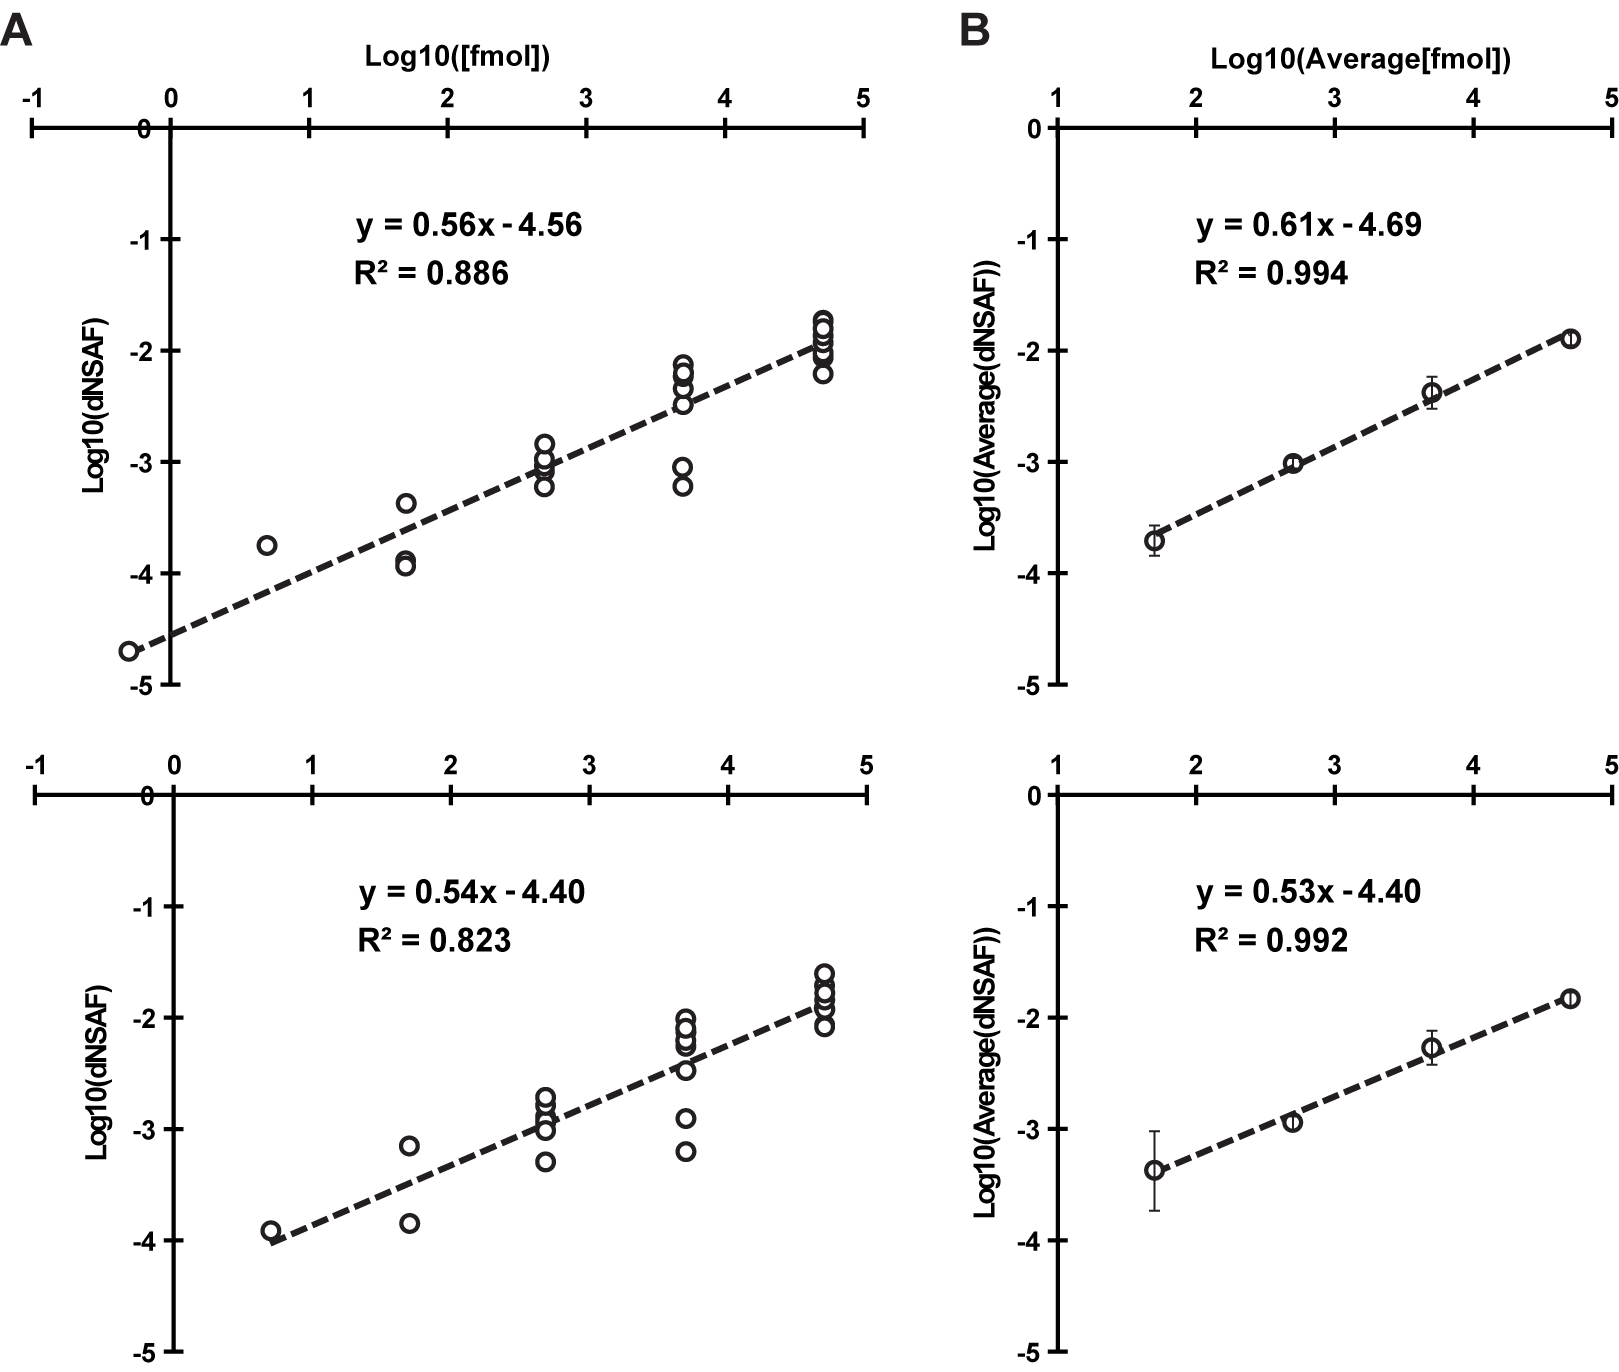
\includegraphics[width=\columnwidth]{MSpC/figure1.png}
	\mycaption{Confirmation of MSpC accuracy by analysis of MS/MS datasets generated with the Universal Proteome Standard 2 (UPS2)}{The array of UPS2 standards were spiked into Xenopus laevis egg \textbf(Top) and embryo \textbf(Bottom) extracts at a range of concentrations.  Following MS/MS analysis, dNSAF values for each protein were determined by Morpheus and MSpC.  \textbf(A) A log-log plot of dNSAF versus concentration for each UPS2 protein detected across each fmol range.  \textbf(B) A log-log plot of average dNSAF vs average concentration of each group of UPS2 proteins at each fmol range: (50, 500, 5000, and 50,000 fmol).}
	\label{fig:UPS2}
\end{figure}

Here, Xenopus egg (see top, Figure \ref{fig:UPS2}) and embryo (bottom, Figure \ref{fig:UPS2}) extracts were spiked at a 4:1 ratio with the Universal Proteome Standard 2 (UPS2), a mix of 48 purified proteins at defined molar ratios of 0.5, 5, 50, 500, 5000, and 50,000, with each ratio containing a different set of 8 of the 48 proteins.
As shown in Figure \ref{fig:UPS2} A, when the Morpheus/MSpC pipeline was used to calculate the average dNSAF value for each UPS2 protein, requiring only a single unique peptide to quantify, strong linear correlations (R$\textsuperscript{2}$ = 0.886 and 0.823) were obtained across a 1,000 fold change in abundance (50 fmol to 50,000 fmol).
In fact, the R$\textsuperscript{2}$ values were similar to those obtained by others with PSM-based LFQ methods \citep{cox14, tu14}.
This linear correlation was further strengthened when the dNSAF values were averaged for all UPS2 proteins within each of the concentration groups, with R$\textsuperscript{2}$ values of 0.994 and 0.992 for the egg and embryo datasets, respectively (see Figure \ref{fig:UPS2} B).
Notably, the slope of the concentration series was significantly less than unity, showing that NSAF measurements are not appropriate for absolute quantification, which was expected given that NSAF is a relative value.  

We also reprocessed the UPS2 dataset using the option of requiring a minimum of two unique peptides for quantification, which should improve stringency.
\begin{figure}[p]
	\centering
	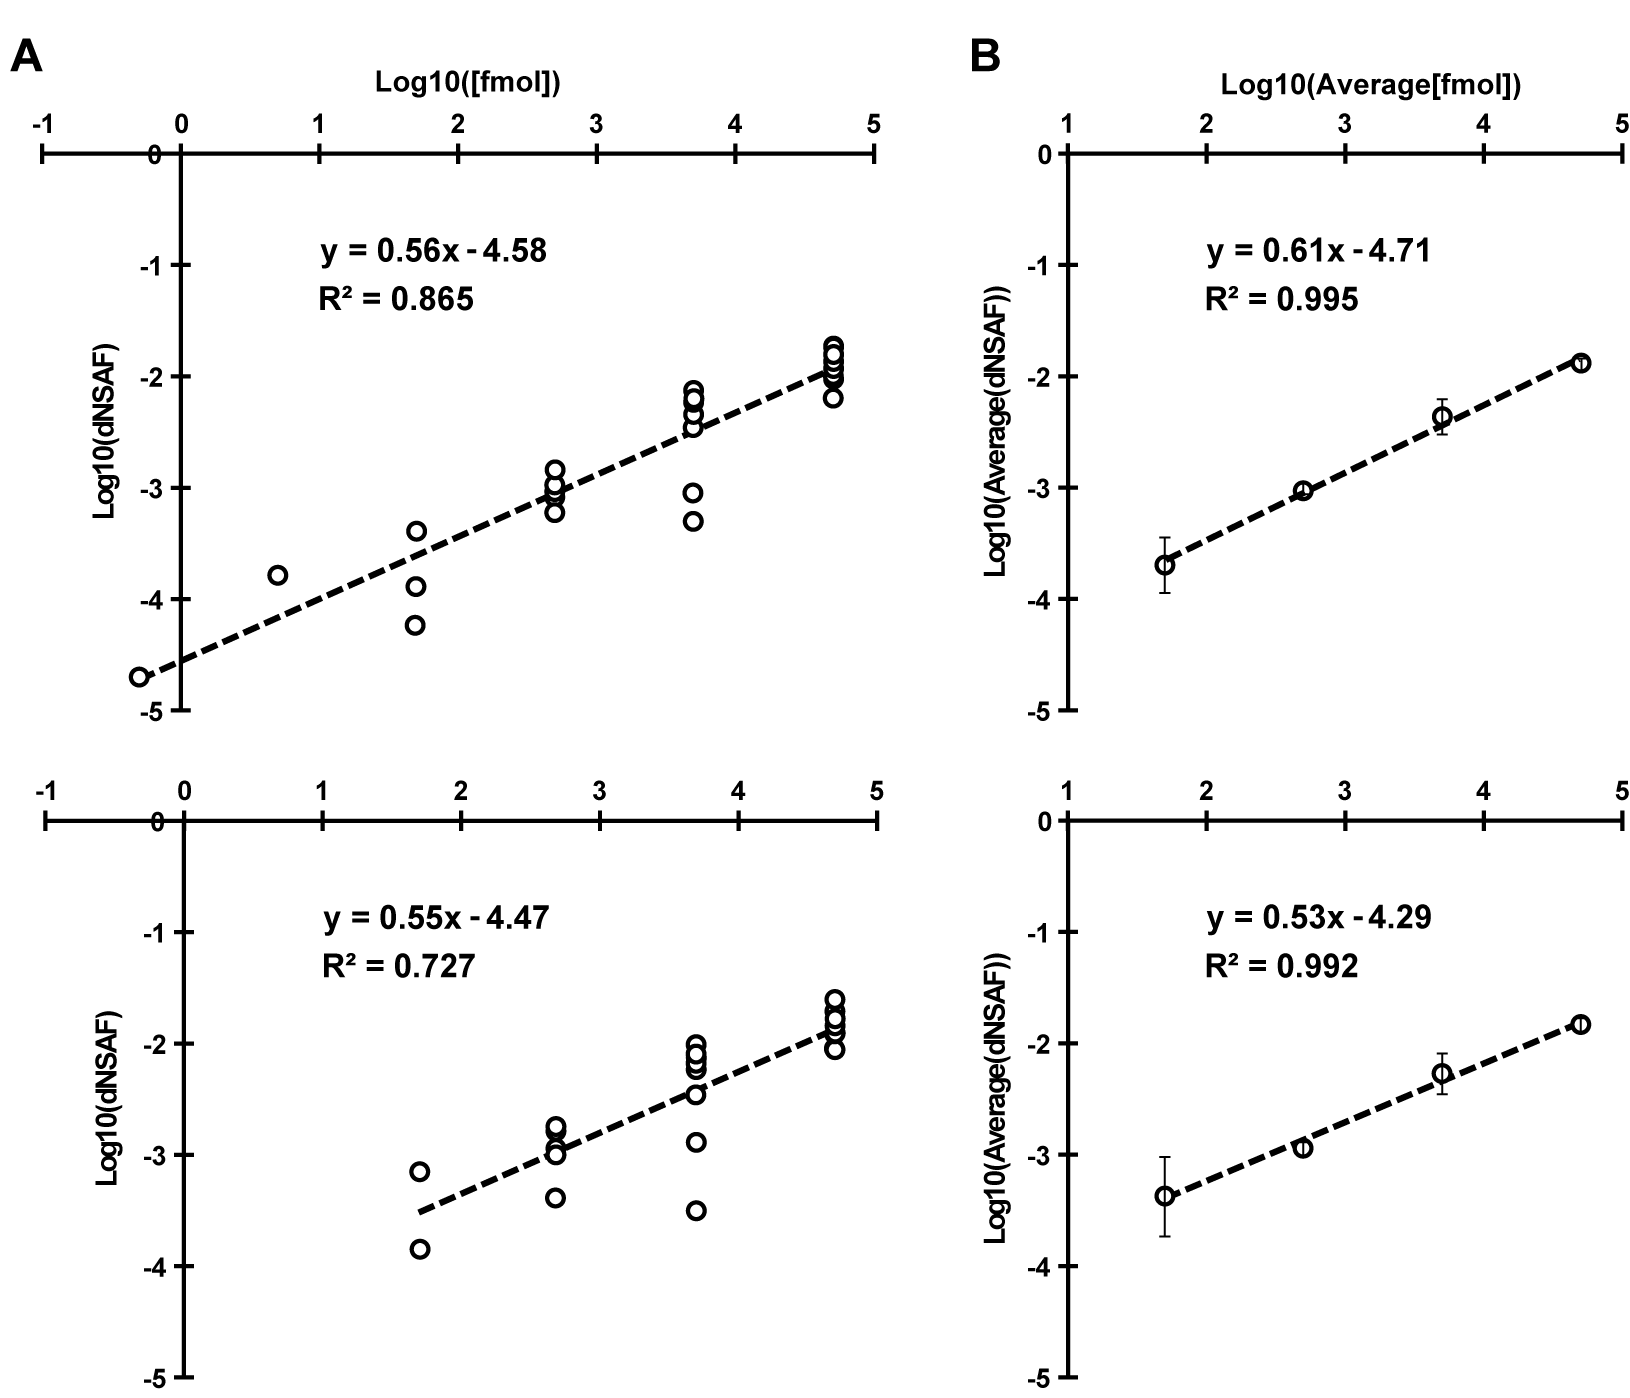
\includegraphics[width=\columnwidth]{MSpC/figure2_supplemental.png}
	\mycaption{Re- Analysis of MS/MS datasets generated with the Universal Proteome Standard 2 (UPS2)}{The array of UPS2 standards were spiked into Xenopus laevis egg \textbf(Top) and embryo \textbf(Bottom) extracts at a range of concentrations.  Following MS/MS analysis, dNSAF values for each protein were determined by Morpheus and MSpC with a change from Figure \ref{fig:UPS2} in that two unique peptides were required to quantify a protein. \textbf(A) A log-log plot of dNSAF versus concentration for each UPS2 protein detected across each fmol range.  \textbf(B) A log-log plot of average dNSAF vs average concentration of each group of UPS2 proteins at each fmol range: (50, 500, 5000, and 50,000 fmol).}
	\label{fig:UPS2twopep}
\end{figure}
This option provided only a minor improvement in overall linearity for the average UPS2 dNSAF values, but decreased linearity when each UPS2 protein was considered individually and removed some UPS2 proteins at low concentrations (compare Figure \ref{fig:UPS2twopep} A to Figure \ref{fig:UPS2} A).
Consequently, caution should be exercised when selecting this option even though it might provide a slight improvement in stringency (see Discussion on Requiring Two Peptide \ref{sec:discussiontwopep}).
To demonstrate the utility and accuracy of MSpC as applied to our work, we analyzed 20S proteasomes isolated from \textit{Arabidopsis thaliana}.
This particle contains multiple subunits assembled in stoichiometric amounts, with many subunits encoded by two paralogous genes of sufficient amino acid identity (typically >90\% \citep{yang04}) such that discrimination between paralogs can be challenging using LFQ approaches \citep{book10}.
To simulate changes in 20S proteasome abundance, we added varying amounts of trypsinized proteasomes (0.05 $\mu$g to 3 $\mu$g) to a fixed amount of trypsinized \textit{Escherichia coli} lysate (0.5 $\mu$g) to generate proteasome/lysate ratios of \textasciitilde0.091, 0.167, 0.333, 0.500, 0.667, 0.750 0.800, 0.857.
The digests were then subjected to MS/MS and the dNSAF value for each subunit along with the uNSAF value for individual isoforms were calculated by the Morpheus/MSpC pipeline (see Methods \ref{sec:methods}).
\begin{FPfigure}[Figure \ref{fig:proteasomespike} \textit{caption follows on next page}]
	\centering
	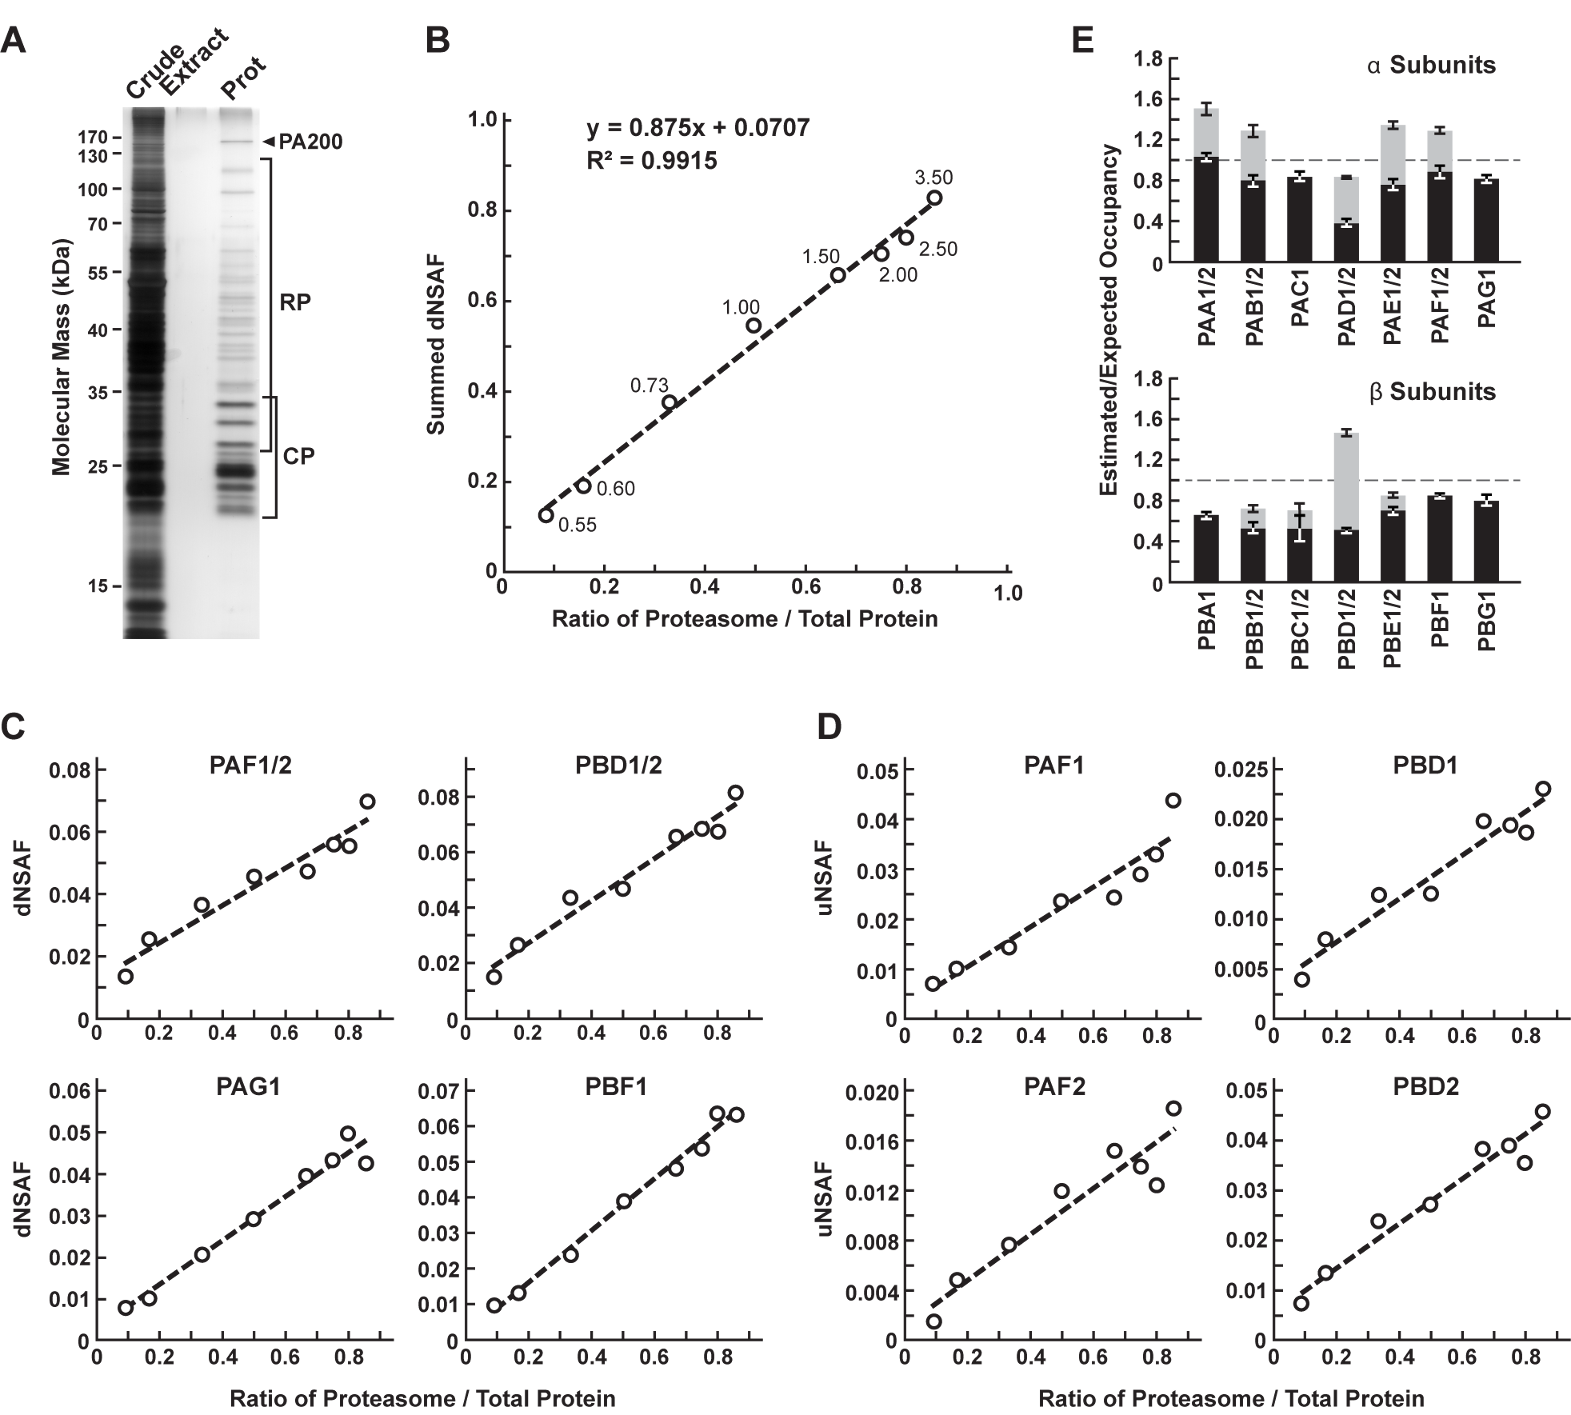
\includegraphics[width=\columnwidth]{MSpC/figure2_rescale.png}
	\mycaption{Confirmation of MSpC accuracy by analysis of MS/MS datasets generated with affinity purified \textit{Arabidopsis} 20S proteasomes spiked into a total cell lysate from \textit{E. coli}. Following MS/MS analysis, the dNSAF and uNSAF values for each subunit/isoform were determined by Morpheus and MSpC}
	{\textbf{(A)} A silver-stained SDS-PAGE gel of 20S proteasome samples affinity purified from 10-d-old \textit{Arabidopsis} seedlings. The crude seedling extract(CE), sample buffer (SB), and affinity-purified 20S proteasome samples (Prot) are shown. \textbf{(B)} Quantification of trypsinized 20S proteasomes when mixed at varying ratios with trypsinized total protein lysates from \textit{E. coli}. The spiked samples were subjected to MS/MS followed by data analysis with the Morpheus and MSpC. dNSAF values for each proteasome subunit were averaged across three technical replicates, then summed to obtain an estimate of abundance for the 20S proteasome, and plotted against their known ratios. The total protein load is listed at each point in ug. \textbf{(C} and \textbf{D)} dNSAF and uNSAF values determined from the data in panel B for individual subunits \textbf{(C)} and their isoforms \textbf{(D)} for several subunits of the 20S proteasome. \textbf{(E)} Quantification accuracy of the Morpheus/MSpC pipeline for determining the amount of each $\alpha$ and $\beta$ subunit of the 20S proteasome. SIngle subunit isoforms are in black, wheras subunits having two isoforms are shown in black and grey to reflect the contributions of isoforms 1 and 2 respectively. Each bar represents the average of eight technical replicates ($\pm$ SE). The dashed line represents the expected value of one assuming an equal stoichiometry of each subunit within the particle.}
	\label{fig:proteasomespike}
\end{FPfigure}
The data from this experiment are deposited in PRIDE with ID PXD003002.
As shown in Figure \ref{fig:proteasomespike}, MSpC provided an excellent determination for the overall abundance of 20S proteasomes within a complex mixture, along with a good reflection of the abundance of individual subunits and their isoforms.

When the dNSAF values for all subunits for the \textit{Arabidopsis} 20S proteasome including their isoforms (representing 14 distinct subunits, 10 of which exist as isoform pairs) were summed, a very close approximation of the dNSAF/actual abundance was obtained (slope=0.875) with a very strong linear correlation (R$\textsuperscript{2}$ = 0.99) over a \textasciitilde10-fold range in protein abundance.  
When each 20S proteasome subunit was analyzed individually, a strong linear response was also obtained (R$\textsuperscript{2}$ > 0.90) for a majority of subunits (Figure \ref{fig:proteasomespike} C and Table \ref{table:MSpC}).

For example, reasonably accurate concentration plots were obtained for the PAF ($\alpha$6) and PBD ($\beta$4) subunits that are encoded by the PAF1/2 and PBF1/2 gene pairs, and for the PAG ($\alpha$7) and PBF ($\beta$6) subunits that are encoded by single PAG1 and PBF1 genes (R$\textsuperscript{2}$  from 0.94 to 0.99).
Even when we calculated uNSAF values for individual isoforms added to the \textit{E. coli} lysate, strong linear responses were obtained (e.g., the PAF1/PAF2 and PBD1/PBD2 pairs) with robust correlations (R$\textsuperscript{2}$ from 0.89 to 0.95) (Figure {fig:proteasomespike} D).
Taken together, MSpC worked well for relative LFQ analysis of a multi-subunit complex and its individual subunits and isoforms within a complex proteomic mixture.

The Morpheus/MSpC pipeline also allowed us to calculate the respective incorporation of each paralog in the complex (see Isoform Incorporation Methods \ref{subsec:isoform}).
As shown in Figure \ref{fig:proteasomespike}E, these estimated/expected occupancies were close to unity for most subunits within both the $\alpha$ and $\beta$ rings of the 20S proteasome.
The only strong deviation was for PBD1/2 ($\beta$4), which  had a greater dNSAF value relative to other $\beta$ subunits across the experiments analyzed (see Table \ref{table:MSpC}).
The calculations for uNSAF values also estimated the relative proportion of each isoform within the complex for those subunits expressed from paralogous genes.
The data obtained are similar to prior studies of the complex involving quantitative top-down proteomic analysis of purified proteasome samples using ultra violet-intrinsic fluorescence to quantify tyrosine-containing subunits \citep{russell13}.
However, our MSpC analysis provided a more complete picture as several subunit isoforms were difficult to quantify by fluorescence either because they lacked tryosine, or because their fluorescence peaks overlapped with those of other subunits/isoforms.
Notably , the protein isoform ratios measured here agree well with the expression ratios for the paralogous genes \citep{book10}, suggesting that the protein isoform abundance generally reflects the relative transcriptional activity of the gene pair.
We consistently estimated slightly more $\alpha$ ring subunits (PAA-PAG) versus $\beta$ ring subunits (PBA-PBG) in the final MSpC calculations (Figure \ref{fig:proteasomespike} E).
This deviation could represent enhanced detection of $\alpha$ ring versus $\beta$ ring subunits, or more likely that purification via the tagged $\alpha$ ring subunit PAG1 also isolated assembly intermediates comprised of only $\alpha$ ring subunits.

We compared the Morpheus and MSpC pipeline to the next most comparable open source, spectral-count-based LFQ pipeline, The Trans Proteomic Pipeline (TPP) \citep{deutsch10} and ABACUS \citep{fermin11} using our datasets generated with the 20S proteasome/\textit{E. coli} lysate mixture (see Tables \ref{table:MSpC} and \ref{table:abacus}).
Morpheus/MSpC slightly outperformed TPP/ABACUS by having a greater overall accuracy (average linearity of 0.88 compared to 0.84), and by having more subunits showing an R$\textsuperscript{2}$ linear correlation greater than 0.9 (14/23 subunits for MSpC versus and 11/23 for ABACUS).
\begin{table}[h]
	\centering
	\mycaption{Table of dNSAF values for each 20S proteasome subunit generated by analyzing the proteasome spike in experiments with the Morpheus and MSpC pipeline}{The top half of the table lists $\alpha$1-7 (PAA-PAG) where 1 or 2 represent different isoforms) subunits, while the bottom half of the table lists $\beta$1-7 subunits (PBA-PBG where 1 or 2 represent different isoforms)}
\npdecimalsign{.}
\nprounddigits{2}
\begingroup
\let\clearpage\relax
\scalebox{0.7}{
\begin{tabular}{|l|l|l|l|l|l|l|l|l|l|l|}
\hline
\textbf{Ratio} & \textbf{0.091} & \textbf{0.167} & \textbf{0.333} & \textbf{0.500} & \textbf{0.667} & \textbf{0.750} & \textbf{0.800} & \textbf{0.857} &                  & \textbf{Pearsons} \\ \hline
PAA1           & 0.0102         & 0.0180         & 0.0275         & 0.0392         & 0.0505         & 0.0489         & 0.0467         & 0.0530         &                  & 0.952             \\ \hline
PAA2           & 0.0063         & 0.0072         & 0.0118         & 0.0121         & 0.0139         & 0.0218         & 0.0351         & 0.0195         &                  & 0.652             \\ \hline
PAB1           & 0.0091         & 0.0117         & 0.0209         & 0.0391         & 0.0377         & 0.0377         & 0.0268         & 0.0397         &                  & 0.721             \\ \hline
PAB2           & 0.0017         & 0.0062         & 0.0147         & 0.0223         & 0.0295         & 0.0277         & 0.0303         & 0.0250         &                  & 0.894             \\ \hline
PAC1           & 0.0076         & 0.0092         & 0.0210         & 0.0339         & 0.0373         & 0.0395         & 0.0546         & 0.0512         &                  & 0.955             \\ \hline
PAD1           & 0.0056         & 0.0070         & 0.0103         & 0.0151         & 0.0160         & 0.0147         & 0.0149         & 0.0147         &                  & 0.826             \\ \hline
PAD2           & 0.0039         & 0.0068         & 0.0141         & 0.0162         & 0.0200         & 0.0225         & 0.0255         & 0.0228         &                  & 0.959             \\ \hline
PAE1           & 0.0046         & 0.0095         & 0.0208         & 0.0352         & 0.0395         & 0.0356         & 0.0389         & 0.0490         &                  & 0.928             \\ \hline
PAE2           & 0.0063         & 0.0082         & 0.0184         & 0.0240         & 0.0269         & 0.0282         & 0.0266         & 0.0293         &                  & 0.925             \\ \hline
PAF1           & 0.0106         & 0.0173         & 0.0239         & 0.0303         & 0.0292         & 0.0379         & 0.0406         & 0.0492         &                  & 0.920             \\ \hline
PAF2           & 0.0032         & 0.0083         & 0.0128         & 0.0155         & 0.0182         & 0.0184         & 0.0152         & 0.0209         &                  & 0.847             \\ \hline
PAG1           & 0.0080         & 0.0100         & 0.0208         & 0.0291         & 0.0394         & 0.0431         & 0.0498         & 0.0423         &                  & 0.966             \\ \hline
               &                &                &                &                &                &                &                &                &                  &                   \\ \hline
\textbf{Ratio} & \textbf{0.091} & \textbf{0.167} & \textbf{0.333} & \textbf{0.500} & \textbf{0.667} & \textbf{0.750} & \textbf{0.800} & \textbf{0.857} &                  & \textbf{Pearsons} \\ \hline
PBA1           & 0.0076         & 0.0104         & 0.0170         & 0.0207         & 0.0246         & 0.0288         & 0.0337         & 0.0449         &                  & 0.898             \\ \hline
PBB1           & 0.0066         & 0.0074         & 0.0191         & 0.0276         & 0.0223         & 0.0206         & 0.0172         & 0.0227         &                  & 0.498             \\ \hline
PBB2           & 0.0009         & 0.0016         & 0.0034         & 0.0035         & 0.0110         & 0.0109         & 0.0160         & 0.0161         &                  & 0.891             \\ \hline
PBC1           & 0.0000         & 0.0000         & 0.0162         & 0.0309         & 0.0373         & 0.0344         & 0.0295         & 0.0388         &                  & 0.877             \\ \hline
PBC2           & 0.0000         & 0.0000         & 0.0000         & 0.0096         & 0.0144         & 0.0147         & 0.0146         & 0.0190         &                  & 0.931             \\ \hline
PBD1           & 0.0053         & 0.0097         & 0.0150         & 0.0147         & 0.0221         & 0.0228         & 0.0231         & 0.0271         &                  & 0.955             \\ \hline
PBD2           & 0.0094         & 0.0162         & 0.0286         & 0.0318         & 0.0426         & 0.0457         & 0.0441         & 0.0538         &                  & 0.969             \\ \hline
PBE1           & 0.0070         & 0.0097         & 0.0156         & 0.0224         & 0.0323         & 0.0373         & 0.0334         & 0.0519         &                  & 0.914             \\ \hline
PBE2           & 0.0007         & 0.0003         & 0.0036         & 0.0069         & 0.0080         & 0.0105         & 0.0106         & 0.0133         &                  & 0.973             \\ \hline
PBF1           & 0.0093         & 0.0122         & 0.0205         & 0.0310         & 0.0368         & 0.0412         & 0.0473         & 0.0459         &                  & 0.991             \\ \hline
PBG1           & 0.0085         & 0.0165         & 0.0203         & 0.0323         & 0.0331         & 0.0345         & 0.0334         & 0.0442         &                  & 0.912             \\ \hline
               &                &                &                &                &                &                &                &                &                  &                   \\ \hline
               &                &                &                &                &                &                &                &                & \textbf{Average} & \textbf{0.885}    \\ \hline
\end{tabular}

}
\endgroup
\npnoround
\label{table:MSpC}
\end{table}
\begin{table}[h]
	\centering
	\mycaption{Table of adj\_NSAF values for each 20S proteasome subunit (equivalent to dNSAF) generated by analzying the proteasome spike in experiments with the TPP and ABACUS pipeline}{The top half of the table lists $\alpha$1-7 (PAA-PAG) where 1 or 2 represent different isoforms) subunits, while the bottom half of the table lists $\beta$1-7 subunits (PBA-PBG where 1 or 2 represent different isoforms)}
\npdecimalsign{.}
\nprounddigits{2}
\begingroup
\let\clearpage\relax
\scalebox{0.7}{
\begin{tabular}{|l|l|l|l|l|l|l|l|l|l|l|}
\hline
\textbf{Ratio} & \textbf{0.091} & \textbf{0.167} & \textbf{0.333} & \textbf{0.500} & \textbf{0.667} & \textbf{0.750} & \textbf{0.800} & \textbf{0.857} &                  & \textbf{Pearsons} \\ \hline
PAA1           & 125.16         & 166.81         & 245.61         & 355.60         & 491.76         & 494.18         & 504.75         & 554.97         &                  & 0.988             \\ \hline
PAA2           & 57.52          & 70.52          & 114.60         & 126.35         & 132.06         & 162.25         & 358.13         & 154.62         &                  & 0.493             \\ \hline
PAB1           & 96.13          & 134.98         & 207.90         & 328.16         & 362.21         & 416.46         & 303.60         & 397.39         &                  & 0.865             \\ \hline
PAB2           & 29.67          & 79.42          & 153.34         & 282.91         & 365.22         & 299.47         & 310.19         & 299.93         &                  & 0.849             \\ \hline
PAC1           & 95.27          & 112.45         & 214.24         & 376.66         & 389.05         & 361.39         & 512.73         & 488.62         &                  & 0.925             \\ \hline
PAD1           & 62.58          & 76.16          & 106.03         & 196.03         & 179.37         & 182.99         & 164.04         & 188.71         &                  & 0.794             \\ \hline
PAD2           & 39.88          & 68.33          & 145.34         & 178.43         & 190.84         & 246.20         & 243.28         & 240.01         &                  & 0.954             \\ \hline
PAE1           & 50.41          & 97.53          & 193.18         & 368.87         & 464.79         & 397.27         & 468.64         & 534.16         &                  & 0.951             \\ \hline
PAE2           & 71.38          & 80.07          & 184.85         & 255.98         & 299.41         & 290.16         & 304.77         & 348.32         &                  & 0.955             \\ \hline
PAF1           & 132.67         & 179.60         & 207.68         & 253.51         & 253.04         & 327.11         & 334.73         & 460.76         &                  & 0.835             \\ \hline
PAF2           & 0.00           & 0.00           & 59.62          & 70.93          & 111.83         & 80.29          & 63.08          & 65.86          &                  & 0.606             \\ \hline
PAG1           & 108.09         & 142.82         & 271.18         & 389.94         & 495.94         & 530.90         & 632.72         & 540.86         &                  & 0.966             \\ \hline
               &                &                &                &                &                &                &                &                &                  &                   \\ \hline
\textbf{Ratio} & \textbf{0.091} & \textbf{0.167} & \textbf{0.333} & \textbf{0.500} & \textbf{0.667} & \textbf{0.750} & \textbf{0.800} & \textbf{0.857} &                  & \textbf{Pearsons} \\ \hline
PBA1           & 85.99          & 113.01         & 208.38         & 233.44         & 273.50         & 327.23         & 417.12         & 560.62         &                  & 0.851             \\ \hline
PBB1           & 47.77          & 80.66          & 195.35         & 324.53         & 303.26         & 220.36         & 200.51         & 216.77         &                  & 0.440             \\ \hline
PBB2           & 17.11          & 4.54           & 0.00           & 0.00           & 21.05          & 102.51         & 144.30         & 187.86         &                  & 0.618             \\ \hline
PBC1           & 27.19          & 40.65          & 165.46         & 345.14         & 364.19         & 386.59         & 338.47         & 373.16         &                  & 0.885             \\ \hline
PBC2           & 10.64          & 40.65          & 0.00           & 55.58          & 145.43         & 158.90         & 159.74         & 228.05         &                  & 0.845             \\ \hline
PBD1           & 50.14          & 94.46          & 168.58         & 167.50         & 244.25         & 248.17         & 252.65         & 319.61         &                  & 0.945             \\ \hline
PBD2           & 81.45          & 149.28         & 256.88         & 319.89         & 390.60         & 407.02         & 380.30         & 490.17         &                  & 0.950             \\ \hline
PBE1           & 81.01          & 107.76         & 196.21         & 302.90         & 365.03         & 404.25         & 378.67         & 441.03         &                  & 0.981             \\ \hline
PBE2           & 0.00           & 1.52           & 5.59           & 8.05           & 40.06          & 56.56          & 59.39          & 58.56          &                  & 0.887             \\ \hline
PBF1           & 71.53          & 112.26         & 190.45         & 226.89         & 259.90         & 366.60         & 431.42         & 420.23         &                  & 0.943             \\ \hline
PBG1           & 104.93         & 174.55         & 232.34         & 392.37         & 425.10         & 397.85         & 396.42         & 463.13         &                  & 0.906             \\ \hline
               &                &                &                &                &                &                &                &                &                  &                   \\ \hline
               &                &                &                &                &                &                &                &                & \textbf{Average} & \textbf{0.845}    \\ \hline
\end{tabular}
}
\endgroup
\npnoround
\label{table:abacus}
\end{table}

In addition to this modest improvement, we note that the Morpheus/MSpC pipeline required significantly less intermediary steps, thus accelerating the data analysis.
Some of the additional steps in TPP/ABACUS could be automated from the command-line, but it would likely be a challenge for the average user.
Importantly, we found that the Morpheus/MSpC pipeline was faster.
Timing tests using the proteasome/\textit{E. coli} spike data generated here showed that the Morpheus/MSpC pipeline was 1.9-fold faster than the TPP/ABACUS pipeline (Figure \ref{fig:MSpCspeed}).
Such an improvement was expected given that Morpheus completes its searches on average 1.3 to 4.6 times faster than most other search engines available \citep{wenger13}. 
Given its simplicity of use, speed, and open source nature, MSpC combined with Morpheus is clearly advantageous over other PSM-based LFQ approaches currently available.  Moreover, by being open source, MSpC should allow others to extend its utility and to serve as a platform for integrating additional open source LFQ approaches into the Morpheus pipeline. 

\begin{figure}[p]
	\centering
	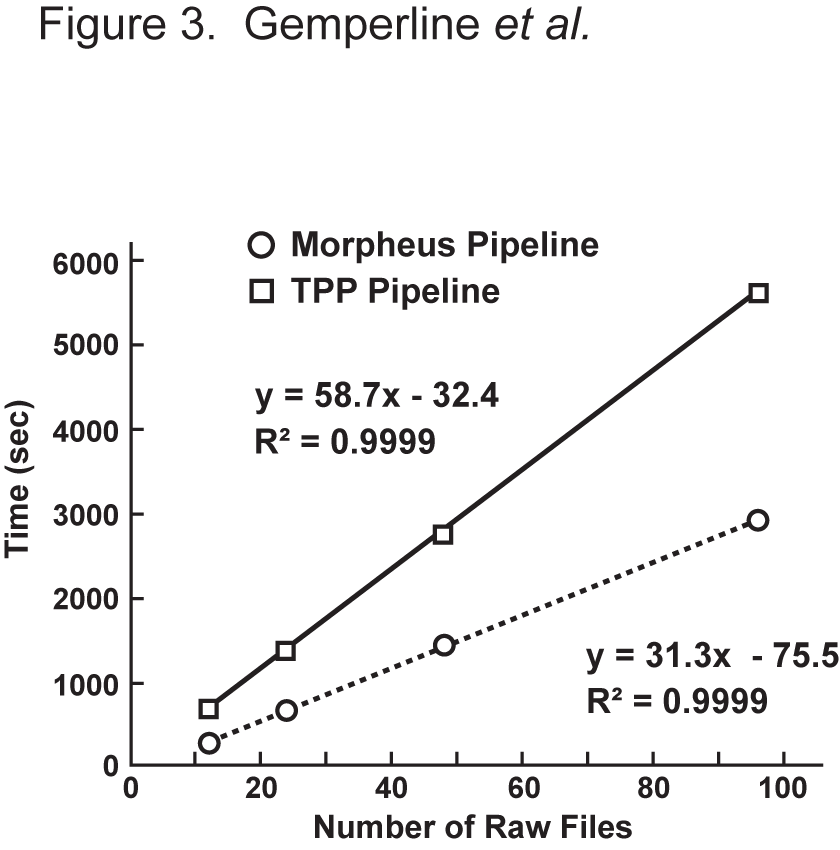
\includegraphics[width=\columnwidth]{MSpC/figure3.png}
	\mycaption{MSpC combined with Morpheus works faster than TPP combined with ABACUS.  Speed comparisons were performed for 12, 24, 48, and 96 raw MS/MS files generated with the 20S proteasome/\textit{E. coli} lysate samples analyzed in \ref{fig:proteasomespike}}{On average, Morpheus/MSpC finished the calculations 1.9 times faster than TPP/ABACUS over a \textasciitilde10-fold range of dataset size.}
	\label{fig:MSpCspeed}
\end{figure}

\section {Methods}
\label{sec:methods}
\subsection{Sample Preparation}

All chemicals were purchased from Sigma-Aldrich unless otherwise stated.  20S proteasomes were obtained as described previously \citep{book10} from \textit{Arabidopsis thaliana} Col-0 ecotype seedlings in which the 20S proteasome subunit PAG1 ($\alpha$7) was genetically replaced with a FLAG-tagged variant, with the minor modification of switching to a more stable HEPES buffer during purification.  The FLAG peptide used for elution was removed by filtering through an Amicon Ultra 4 10K filter with the elution buffer also exchanged into 8 M urea.  Total protein was quantified by the bicinchoninic acid protein assay (Thermo Scientific) using bovine serum albumin as the standard.  Approximately 70 $\mu$g of proteasomes were digested overnight at 37$^\circ$C using a 1:30 trypsin/sample ratio.  Peptides were acidified to a final concentration of 1\% TFA, desalted on a Waters C18 Sep-Pak containing 50 mg sorbent material, and lyophilized.  Total \textit{E coli} lysates were obtained from Bio-Rad (Cat. 163-2110) with 200 $\mu$g digested as above.  Both proteasome and \textit{E. coli} peptides were dissolved in 5\% acetonitrile, 95\% water, and 0.1 \% formic acid.  Each MS analysis, performed in triplicae, used 5 $\mu$L volumes prepared with 3, 2, 1.5, 1, 0.5, 0.25, 0.1, or 0.05 $\mu$g of digested proteasomes mixed with 0.5 $\mu$g of digested E. c.oli proteins.  This mixtures reflected proteasome/\textit{E. coli} ratios of \textasciitilde0.091, 0.167, 0.333, 0.500, 0.667, 0.750 0.800, and 0.857, respectively.

\subsection{Liquid Chromatography and High-Resolution Mass Spectrometry}

Samples were analyzed by ultra-high performance liquid chromatography (UPLC) (nanoAcquity, Waters Corporation) connected online to an electrospray ionization LTQ Velos Orbitrap mass spectrometer (Thermo Scientific).  Separation employed a 100 x 365 $\mu$m fused silica capillary micro-column packed with 20 cm of 1.7 $\mu$m-diameter, 130-$\AA$ pore size, C18 beads (Waters BEH), with an emitter tip pulled to approximately 1 $\mu$m using a laser puller (Sutter Instruments).  Peptides were loaded at a flow-rate of 400 nL/min for 30 min and then eluted over 120 min at a flow-rate of 300 nL/min with a 2\% to 30\% acetonitrile gradient in 0.1\% formic acid.  Full-mass scans were performed in the FT Orbitrap with a mass range of 300-1500 m/z at a resolution of 60,000, followed by ten MS/MS high energy C-trap dissociation scans of the ten highest intensity parent ions at 42\% normalized collision energy and 7,500 resolution, with a mass range starting at 100 m/z.  Dynamic exclusion was enabled with a repeat count of two over the duration of 30 sec and an exclusion window of 120 sec.  

\subsection{Data Processing}

Protein identifications were determined using the Morpheus search engine \citep{wenger13}.  Raw data was searched with the Thermo module of Morpheus revision 151 downloaded and compiled from source code available at \url{http://sourceforge.net/projects/morpheus-ms/} using Microsoft Visual Studio 2013 professional edition.  The following parameters were used to search all databases: unknown precursor charge states - +2, +3, +4; maximum number of MS/MS peaks = 400; assign charge states - enabled; de-isotope - disabled; generate target decoy database on the fly; protease trypsin (no proline rule); maximum missed cleavages = 2; initiator methionine behavior - variable; fixed modification of carbamidomethylation of cysteine; variable modification of oxidation of methionine; maximum variable modification isoforms per peptide = 1024; precursor mass tolerance = $\pm$ 2.1 Da monoisotopic (recommended parameters to account for neutral loss); precursor monoisotopic peak correction - disabled; product mass tolerance = $\pm$ 0.025 Da monoisotopic; consider modified forms as unique peptides - false; maximum threads = 8; minimize memory usage - false.   
MSpC quantification of Universal Proteome Standard 2 (UPS2) protein sequences exploited the MS/MS analysis of individual USP2 proteins (Sigma-Aldrich) mixed at various concentrations with egg or embryo extracts from Xenopus laevis available in the PRoteomics IDEntifications (PRIDE) repository \citep{vizcaino13} using identifier - PXD000902 and the available proteomics database - pita\_v1.71.protein.name.fa.  For our analysis, both the raw MS/MS data and resulting FASTA files for the USP2 and egg and embryo proteomes were obtained from PRIDE.  The database used for searching the MS/MS data of \textit{Arabidopsis} proteasomes spiked into total \textit{E. coli} peptides was generated by combining Uniprot K12 \textit{E. coli} reference proteome UP000000625 with a common contaminant database, and then mixing the merged dataset with FASTA sequences for all proteoforms of all known proteasome subunits and associated proteins \citep{book10} obtained from the TAIR10\_pep\_20101214 FASTA database available within The \textit{Arabidopsis} Information Resource (TAIR) version 10.  All FASTA files are available for download in the Supporting Information.  The datasets were analyzed by MSpC with a 1\% PSM false discovery rate (FDR) and a 1\% protein group FDR to determine NSAF, dNSAF, and uNSAF values for each protein group. Two separate analyses were performed in which one unique, or alternatively two unique peptides were required to quantify a protein group.  NSAF values were calculated according to formulas 1a, 2a, and 3a from Figure 1 of Zhang et al. \citep{zhang10}.

\subsection {Isoform Incorporation Rates}
\label{subsec:isoform}
	For the individual subunit analysis of the 20S proteasome the isoform incorporation rates were treated as follows. Given that each proteasome subunit should be incorporated at equal stoichiometry within the 20S particle, we then tested whether the Morpheus/MSpC pipeline could calculate the relative abundance of each subunit and the distribution of isoforms.  Here, we divided the dNSAF values for each subunit/isoform by the total number of dNSAF values for the entire complex across all eight total proteasome/\textit{E. coli} lysate ratios tested.  This averaged value provided a concentration-independent ratio for the incorporation of each subunit/isoform.  We then normalized these values based on a 1/14 stoichiometry of each subunit within the complex to calculate the estimated occupancy versus the expected occupancy of each subunit.  

\subsection{Speed and Accuracy Comparisons of Morpheus/MSpC to the TPP/ABACUS Pipeline}

The speed and accuracy of MSpC combined with Morpheus was compared to the next most comparable open source software suite for calculating NSAF values; i.e., TPP \citep{deutsch10} combined with ABACUS \citep{fermin11}, using the proteasome spike-in experiment files as input.  The .raw files were converted to .mzmL files by TPP Build 201411201551-6764 and then searched using the multi-threaded X!Tandem MS/MS search engine \citep{craig04} with the search parameters adjusted as close as possible to that used for the Morpheus searches.  A decoy database was generated using the TPP tool DecoyFASTA for use with X!Tandem.  Relevant  X!Tandem parameters are listed here: parent monoisotopic mass error = $\pm$ 2.1 Da, fragment mass error = $\pm$ 0.025 Da, fixed modifications of carbamidomethylation (57.021464) on cysteine, and variable modification of oxidation (15.994915) on methionine, fully tryptic cleavages, missed cleavage sites = 2 maximum, no refinement and 8 threads.  The configuration file used and the test datasets can be found in the Supporting Information. The data were analyzed in the TPP using Peptide Prophet \citep{keller02}.  Relevant settings are listed: minimum probability = 0.05; minimum peptide length = 7; accurate mass, and nonparametric decoy database to pin down false discovery rate; ignore +1 charged spectra; and run Protein Prophet \citep{nesvizhskii03} after Peptide Prophet.  
Once completed, all pepxml data from Peptide Prophet contained in a single folder was combined using the command line version of Protein Prophet from the TPP binaries with the following command: ProteinProphet.exe *.pep.xml interact-COMBINED.prot.xml.  This post-analysis aggregation was required for running the spectral counting program ABACUS.  Here, we note that there are no graphic user interfaces to perform this post analysis aggregation, which makes this portion of the data analysis more difficult for those unfamiliar with setting up and running programs from the command line.  The combined data was analyzed by ABACUS with the following parameters: best peptide probability = 0.99; minimum peptide probability = 0.99; experimental peptide probability = 0; and combined file probability = 0.99 to most accurately match a 1\% FDR stringency settings in MSpC.  dNSAF values were compared in Microsoft Excel using the CORREL function and squaring the result.  Additional timing tests were performed with a subset of the calibration curve data (ratios 0.091, 0.167, 0.333, and 0.500 in triplicate corresponding to 12 .raw files) by increasing file input to 24 (2x), 48 (4x), and 96 (8x) .raw files to determine the time dependence on input size between both pipelines tested (Morpheus/MSpC versus TPP/ABACUS).  The timing tests and all data analyses were performed on a computer running Windows 7 Ultimate, with 16 GB of random access memory, and an Intel Core i7-2700k with hyper-threading turned on for eight logical cores.

\section {Discussion on Requiring Two Unique Peptides to Quantify a Protein}
\label{sec:discussiontwopep}
Occasionally, some researchers may want to use a more stringent criterion for quantification such as requiring a protein to have more than one unique identifying peptide. To see how this might affect our data analysis, we re-analyzed our results shown in Figure \ref{fig:UPS2twopep}, this time requiring two unique peptides to quantify an individual protein. The results point to a very small increase in linearity observed in the average plots; however, there is a slight decrease in linearity for the egg sample (0.886 to 0.865) and a larger decrease in linearity for the individual UPS2 protein plot for the embryo sample (0.827 to 0.723). The decrease in linearity in the embryo sample is due to the analysis removing a low abundance UPS2 protein (O00762ups) identified with only one unique peptide. While some have suggested that requiring more than one unique peptide to identify a protein is an ideal approach, requiring two peptides for identifications in database searches reduces the number of protein identifications in the target database more than those in the decoy database and results in increased false discovery rates . While we recognize that researchers may want to implement more stringent requirements than what is typically used in database searching to quantify a set of proteins, there are two cases where requiring two unique peptides may not be ideal in a quantitative analysis. Firstly, low abundance proteins that have few PSMs might be identified by only a single peptide and thus be erroneously thrown out of the analysis. Secondly, there may be only one unique peptide that can differentiate between families of homologous proteins. In this second case, requiring two unique peptides would remove these homologous proteins from the MSpC analysis, even if they had a large number of PSMs. Because of these reasons and because of the decreased linearity observed when requiring proteins to have two unique peptides (Figure \ref{fig:UPS2twopep}) as compared to one unique peptide (Figure \ref{fig:UPS2}), we suggest caution in requiring more than one unique peptide per protein.

\section {Tutorial}
\label{sec:tutorial}

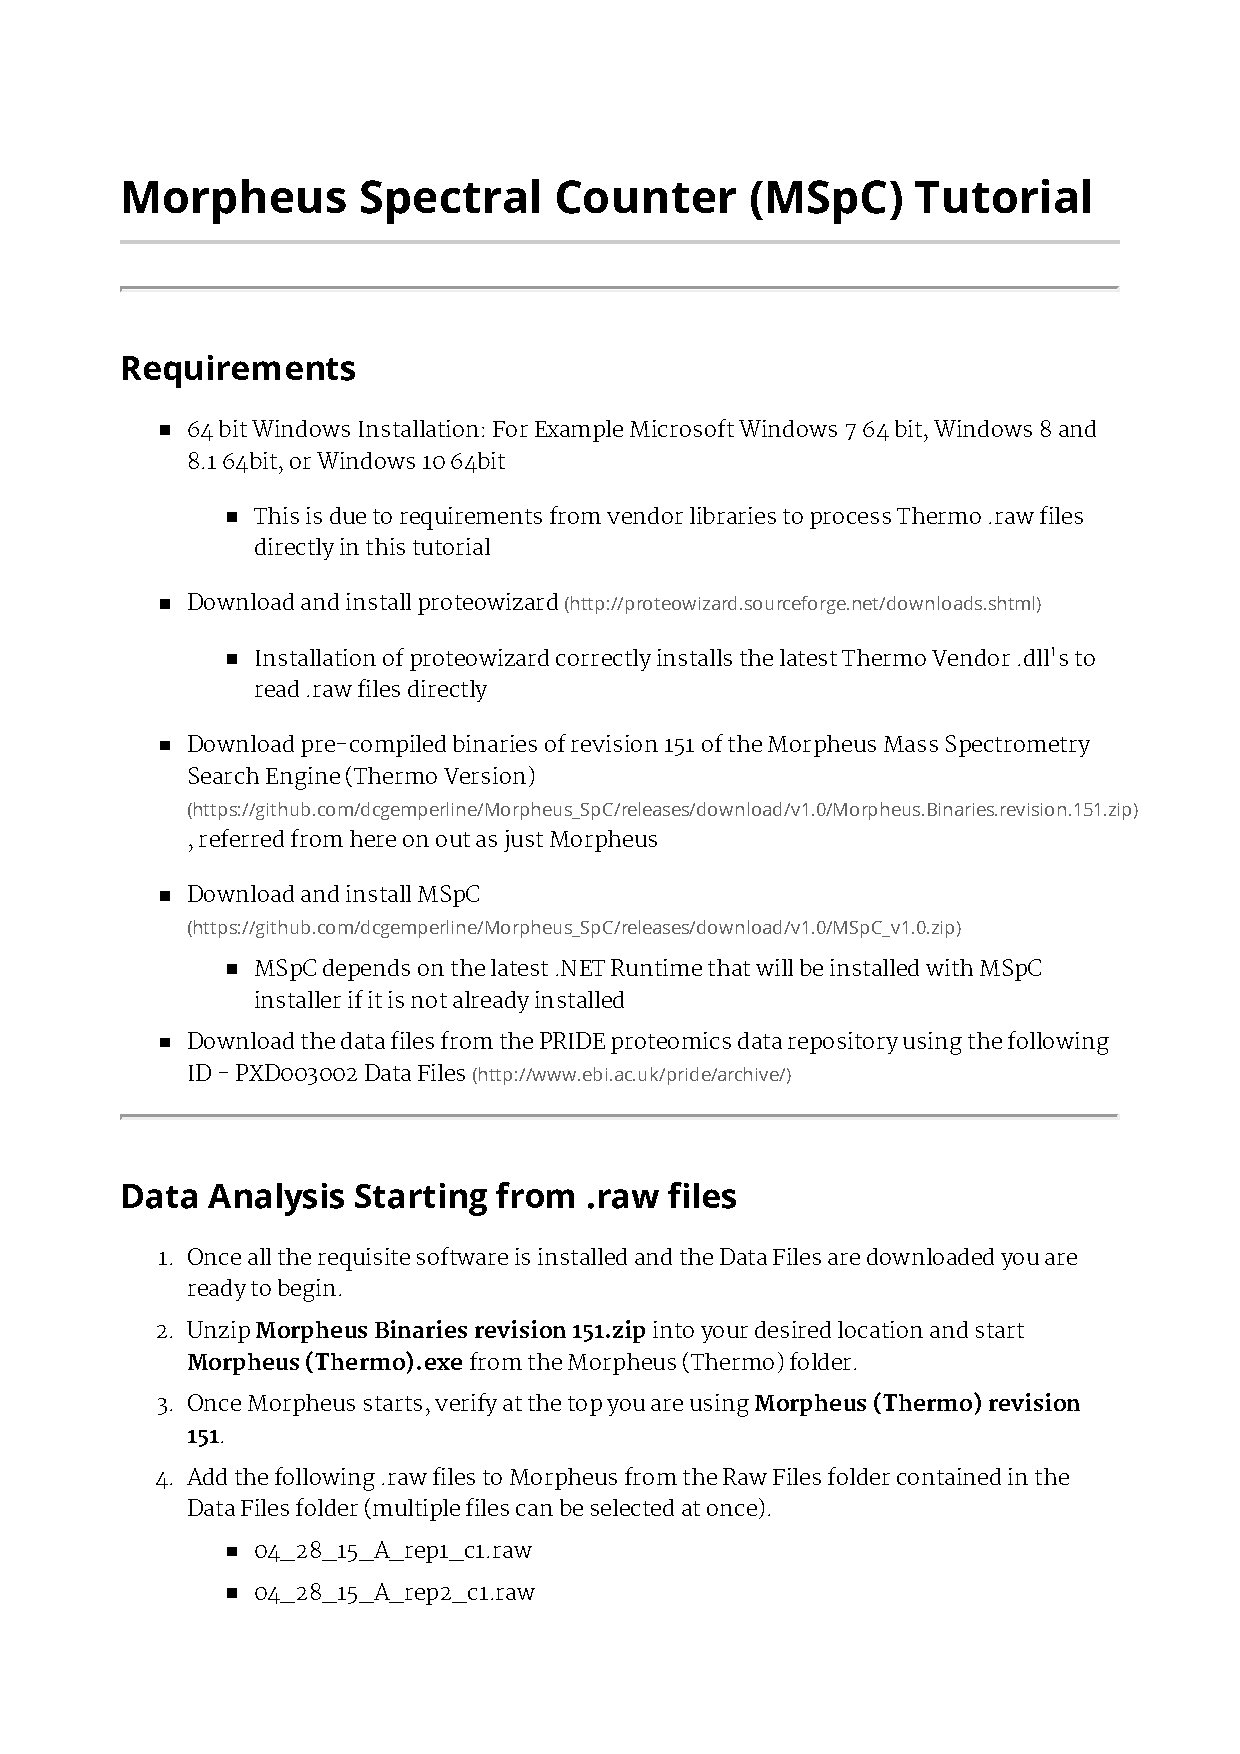
\includepdf[pages=-]{MSpC/Tutorial.pdf}


\section {Acknowledgements}
D.C.G. was supported by a grant from the U.S. Department of Energy Office of Science; Office of Basic Energy Sciences; Chemical Sciences, Geosciences, and Biosciences Division (DE-FG02-88ER13968) and a graduate training fellowship from the NIH (5 T32 GM 7133-37).  M.S. and L.M.S were supported by a grant from the National Institute of Health/National Institute of General Medical Sciences (1P50HG004942).  The authors thank Erin Gemperline, Richard S. Marshall, and Josh Coon for critical reading of the manuscript, and additionally thank Derek Bailey for a critical code review.

\bibliographystyle{plantcell2}
\bibliography{MSpC}
